\chapter{Numerical Results}\label{ch4}

In this section, we will show our approximation results for mean-reverting CEV model and Heston plus CEV model, expansion of mispricing functions is up to $N=3$. We utilize a symbolic library of \footnote{Codes used for this paper can be accessed through my   \href{https://github.com/ywang408/master-thesis-code}{Github}}{python} \href{https://www.sympy.org/en/index.html}{sympy} to calculate expansions, and use Monte Carlo simulations with 200 time steps and 100000 paths as our benchmark because there's no existing pricing formula for these models. We evaluate the accuracy of our results with two kinds of figures, the first kind is the direct comparison between benchmarks and our approximation results, the second one is the relative differences between benchmarks and our results. Besides, we also have attached detailed results in the Appendix \ref{mrcev}.

\section{Volatility option prices under mean-reverting CEV model}

For options under mean-reverting CEV model,

$$
  \begin{cases}
    d V_t=\kappa(m- V_t) d t+\sigma_{\text{CEV}} V^{\gamma}_t d W_t &\text{true model}\\
    d V_t=\kappa(m - V_t) d t+\sigma_0 \sqrt{V_t} d W_t &\text{auxiliary model}
  \end{cases}
$$

We use the same mean-reverting parameters as \cite{grunbichler_valuing_1996} used in his model, the parameters are $\kappa=4$, $\theta=15$. Besides, we set the nuisance parameter $\sigma_0 = \sigma_{\text{CEV}} V_0^{\gamma-\frac{1}{2}}$, where $V_0=V(t)$ is the initial value of volatility at start point $t$. We test our approximation method with different constant elasticity parameters, the main idea of setting these parameters is that for small $\gamma$, which enlarges the importance of $V$ in the CEV part, we use a small $\sigma$; Whereas for large $\gamma$ we set a large $\sigma$. 

\begin{figure}[ht]
  \centering
  \subfloat[price comparison with $\tau=0.1$]{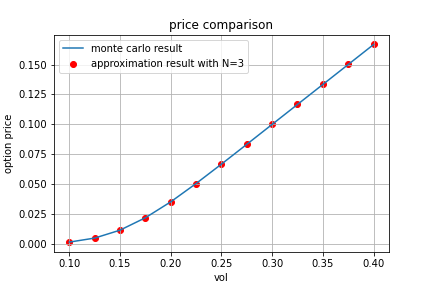
\includegraphics[width=0.5\textwidth]{./figures/T=0.1,K=0.15, kappa=4,m=0.15, sigma=0.15, gamma=0.15 price.png}\label{price comparison1}}
  \hfill
  \subfloat[relative error with $\tau=0.1$]{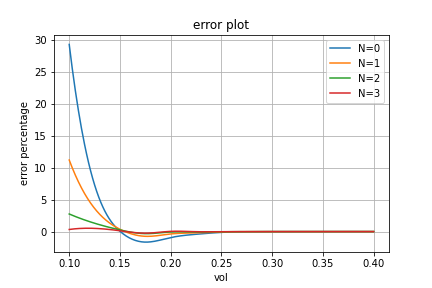
\includegraphics[width=0.5\textwidth]{./figures/T=0.1,K=0.15, kappa=4,m=0.15, sigma=0.15, gamma=0.15 error.png}\label{price diff1}} \\
  \subfloat[price comparison with $\tau=0.3$]{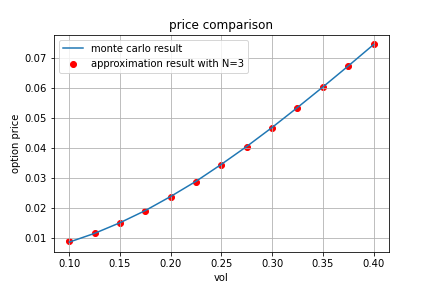
\includegraphics[width=0.5\textwidth]{./figures/T=0.3,K=0.15, kappa=4,m=0.15, sigma=0.15, gamma=0.15 price.png}\label{price comparison2}}
  \hfill
  \subfloat[relative error with $\tau=0.3$]{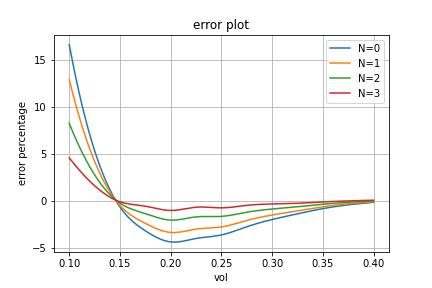
\includegraphics[width=0.5\textwidth]{./figures/T=0.3,K=0.15, kappa=4,m=0.15, sigma=0.15, gamma=0.15 error.png}\label{price diff2}} \\
  \subfloat[price comparison with $\tau=0.5$]{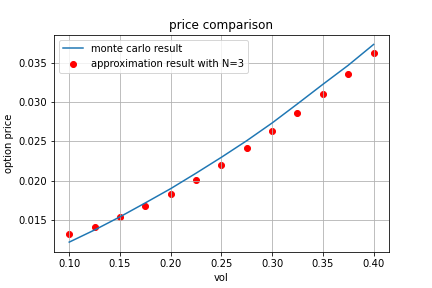
\includegraphics[width=0.5\textwidth]{./figures/T=0.5,K=0.15, kappa=4,m=0.15, sigma=0.15, gamma=0.15 price.png}\label{price comparison3}}
  \hfill
  \subfloat[relative error with $\tau=0.5$]{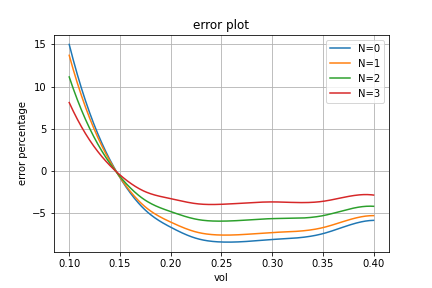
\includegraphics[width=0.5\textwidth]{./figures/T=0.5,K=0.15, kappa=4,m=0.15, sigma=0.15, gamma=0.15 error.png}\label{price diff3}}
  \caption{mean-reverting CEV model result 1}
  \small{Parameters are $K=0.15, \kappa=4, m=0.15, \sigma=0.15, \gamma=0.15$}
  \label{mrcev res1}
\end{figure}

For figure \ref{mrcev res1}, our parameters are $\sigma=0.15$, $\gamma=0.15$, and with different maturities $\tau=0.1$, $\tau=0.3$, $\tau=0.5$. We can find that in \ref{price comparison1}, \ref{price comparison2} and figure \ref{price comparison3} our approximation results with expansion order $N=3$ are very accurate. Figure \ref{price diff1}, figure \ref{price diff2} and figure \ref{price diff3} show the relative error with different expansion orders. We can find that the results with $N=3$ outperform other results, which implies that keep applying Ito-Taylor expansions on the mispricing functions can create increasingly improved refinements and provide us with more and more accurate results.

Parameters for figure \ref{mrcev res2} are $\sigma=0.6$, $\gamma=0.75$, and with different maturities $\tau=0.1$, $\tau=0.3$, $\tau=0.5$, other parameters keep the same. Similarly, our method still provide accurate results.

\begin{figure}[t]
  \centering
  \subfloat[price comparison with $\tau=0.1$]{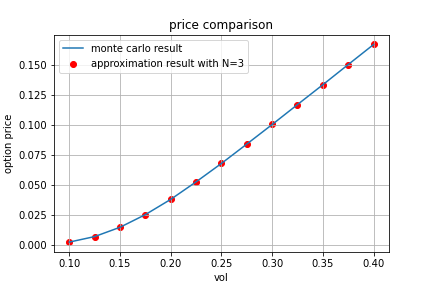
\includegraphics[width=0.5\textwidth]{./figures/T=0.1,K=0.15, kappa=4,m=0.15, sigma=0.6, gamma=0.75 price.png}\label{price comparison4}}
  \hfill
  \subfloat[relative error with $\tau=0.1$]{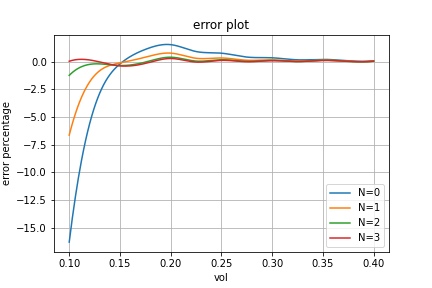
\includegraphics[width=0.5\textwidth]{./figures/T=0.1,K=0.15, kappa=4,m=0.15, sigma=0.6, gamma=0.75 error.png}\label{price diff4}} \\
  \subfloat[price comparison with $\tau=0.3$]{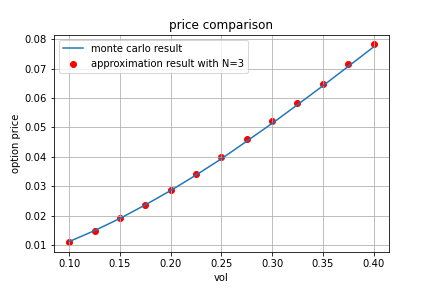
\includegraphics[width=0.5\textwidth]{./figures/T=0.3,K=0.15, kappa=4,m=0.15, sigma=0.6, gamma=0.75 price.png}\label{price comparison5}}
  \hfill
  \subfloat[relative error with $\tau=0.3$]{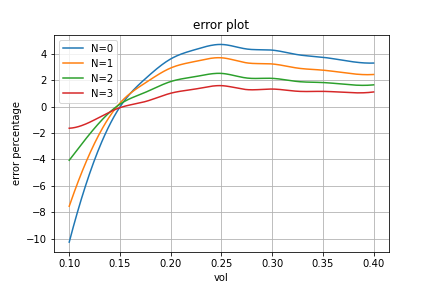
\includegraphics[width=0.5\textwidth]{./figures/T=0.3,K=0.15, kappa=4,m=0.15, sigma=0.6, gamma=0.75 error.png}\label{price diff5}} \\
  \subfloat[price comparison with $\tau=0.5$]{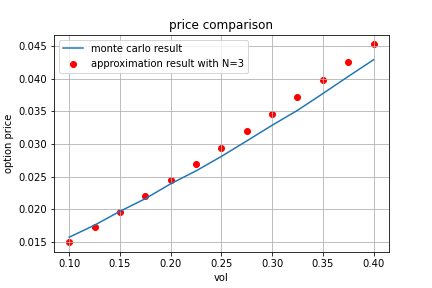
\includegraphics[width=0.5\textwidth]{./figures/T=0.5,K=0.15, kappa=4,m=0.15, sigma=0.6, gamma=0.75 price.png}\label{price comparison6}}
  \hfill
  \subfloat[relative error with $\tau=0.5$]{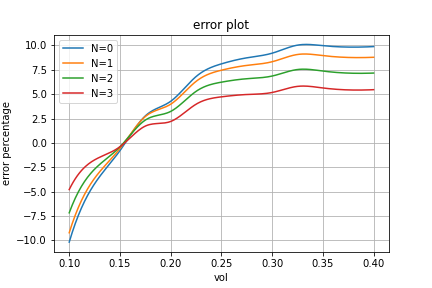
\includegraphics[width=0.5\textwidth]{./figures/T=0.5,K=0.15, kappa=4,m=0.15, sigma=0.6, gamma=0.75 error.png}\label{price diff6}}
  \caption{mean-reverting CEV model result 2}
  \small{Parameters are $K=0.15, \kappa=4, m=0.15, \sigma=0.6, \gamma=0.75$}
  \label{mrcev res2}
\end{figure}

One may observe that when KM use Black-Scholes model as auxiliary model to price options under Heston model, for deep in-the-money options, relative differences always converge to 0 no matter how many orders of expansions are applied. That is because in his case delta of option is very close to 1 and Vega is close to 0, which means option prices are mainly driven by underlying stocks' prices, and volatility has no influence on option prices. Besides, using Black-Scholes model makes mispricing function depend on gamma, while gamma of deep in-the-money options is also close to 0, meaning that their mispricing functions don't affect option prices at all. As a result, their figures show that all results' relative errors are converging to 0 as stock price increases.

However, in our model, underlying assets follow mean-reverting CEV model. \cite{grunbichler_valuing_1996} mention that when volatility $V$ is above its long-term mean, mean-reversion property implies the expected future value of V will be lower than its current value, making the expected payoff for a volatility call can be less than its current intrinsic value. The property of options under Black-Scholes world doesn't hold here, recall that before we set $\sigma_0 = \sigma_{\text{CEV}}V_0^{\gamma-\frac{1}{2}}$. Obviously when $V_0$ is relatively large, $\sigma_{\text{CEV}} V^{\gamma}_t > \sigma_{\text{CEV}}V_0^{\gamma-\frac{1}{2}} \sqrt{V}_t$, causing the loss of accuracy in our auxiliary model. It gives an explanation why the relative error of our method converges to slightly smaller than 0 for deep in-the-money options. 

Besides, we notice that for results with $\tau=0.5$, our results sometimes seem not accurate enough. Though in figure \ref{mrcev res1}, figure \ref{mrcev res2}, relative differences reduce as we apply higher order expansions. We may predict that if applying further expansions we could get more precise results. However, this raises a constraint of KM's method, number of terms grow exponentially in the final pricing formula as we keep expanding mispricing functions, causing the running time of calculation increasing dramatically, which is a trade-off between applying high order expansions and getting more accurate results. Therefore, if we still don't get a desired result with a threshold expansion order, say $N=5$, we may need to reconsider our auxiliary models and nuisance parameters. In our case, we can take the advantage of volatility following mean-reverting process, for $\tau>0.5$, we set nuisance parameter $\sigma_0 = \sigma_{\text{CEV}}m^{\gamma-\frac{1}{2}}$. Results are accurate again and shown in figure \ref{mrcev res t}.

\begin{figure}[t]
  \centering
  \subfloat[price comparison with $\tau=0.5, \sigma=0.15, \gamma=0.15$]{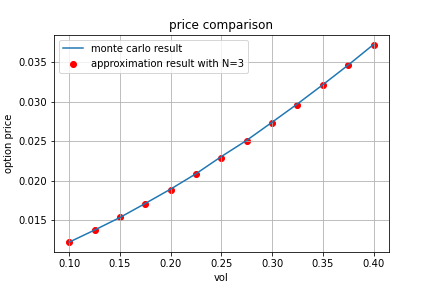
\includegraphics[width=0.5\textwidth]{./figures/t>0.5/,K=0.15, kappa=4,m=0.15, sigma=0.15, gamma=0.15v2 price.png}\label{price comparison l1}}
  \hfill
  \subfloat[relative error with $\tau=0.5, \sigma=0.15, \gamma=0.15$]{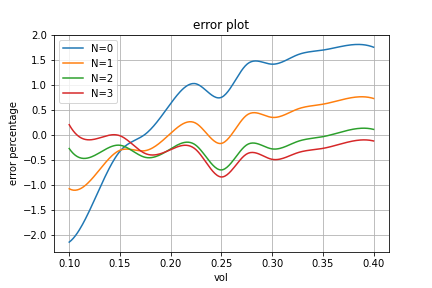
\includegraphics[width=0.5\textwidth]{./figures/t>0.5/,K=0.15, kappa=4,m=0.15, sigma=0.15, gamma=0.15v2 error.png}\label{price diff l1}} \\
  \subfloat[price comparison with $\tau=0.5, \sigma=0.6, \gamma=0.75$]{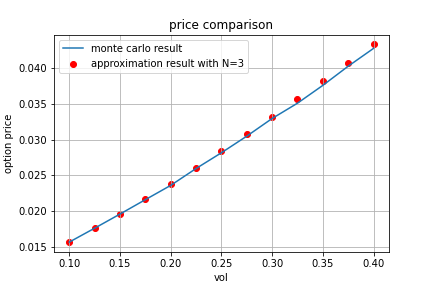
\includegraphics[width=0.5\textwidth]{./figures/t>0.5/,K=0.15, kappa=4,m=0.15, sigma=0.6, gamma=0.75v2 price.png}\label{price comparison l2}}
  \hfill
  \subfloat[relative error with $\tau=0.5,\sigma=0.6, \gamma=0.75$]{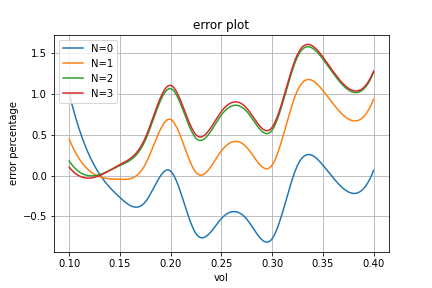
\includegraphics[width=0.5\textwidth]{./figures/t>0.5/,K=0.15, kappa=4,m=0.15, sigma=0.6, gamma=0.75v2 error.png}\label{price diff l2}} \\
  \caption{mean-reverting CEV model result with $\tau=0.5$ and new nuisance parameter}
  \small{Other parameters are $K=0.15, \kappa=4, m=0.15$}
  \label{mrcev res t}
\end{figure}

Additionally, using our method to price options with very small value can also be challenging. The loss of accuracy for approximating non-central chi-square distribution functions would be magnified under this condition. In figure \ref{mrcev res3}, our parameters for mean-reverting CEV model are $\kappa=6, m=0.06, \sigma=1.4, \gamma=1.2$. Because we uses a small long-term mean parameter $m=0.06$, when time to maturity increases, volatility value $V$ will less than $K=0.15$. In this case, volatility option price would have small value, which magnifies our other errors.

\begin{figure}[t]
  \centering
  \subfloat[price comparison with $\tau=0.1$]{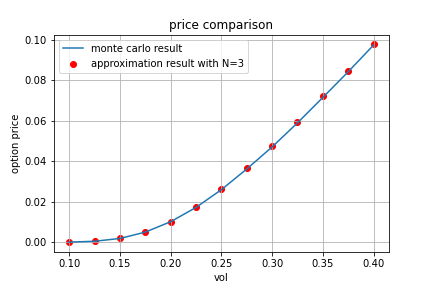
\includegraphics[width=0.5\textwidth]{./figures/T=0.1,K=0.15, kappa=6,m=0.06, sigma=1.4, gamma=1.2 price.png}\label{price comparison7}}
  \hfill
  \subfloat[relative error with $\tau=0.1$]{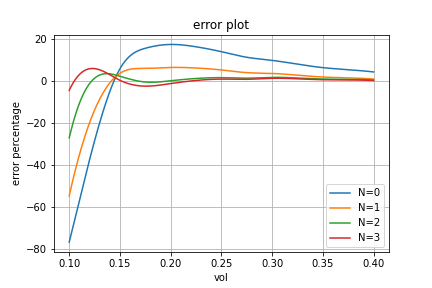
\includegraphics[width=0.5\textwidth]{./figures/T=0.1,K=0.15, kappa=6,m=0.06, sigma=1.4, gamma=1.2 error.png}\label{price diff7}} \\
  \subfloat[price comparison with $\tau=0.3$]{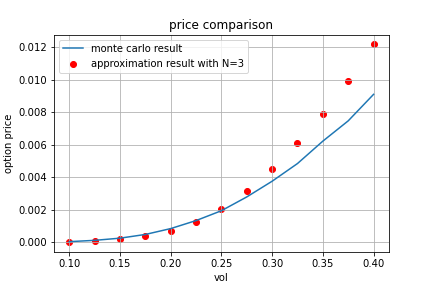
\includegraphics[width=0.5\textwidth]{./figures/T=0.3,K=0.15, kappa=6,m=0.06, sigma=1.4, gamma=1.2 price.png}\label{price comparison8}}
  \hfill
  \subfloat[relative error with $\tau=0.3$]{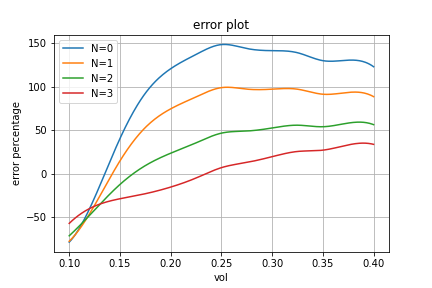
\includegraphics[width=0.5\textwidth]{./figures/T=0.3,K=0.15, kappa=6,m=0.06, sigma=1.4, gamma=1.2 error.png}\label{price diff8}} \\
  \subfloat[price comparison with $\tau=0.5$]{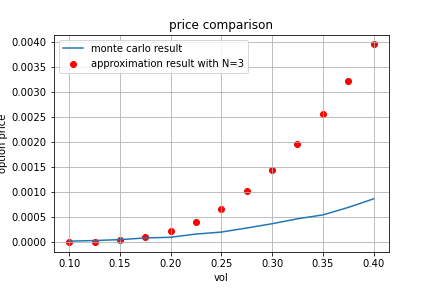
\includegraphics[width=0.5\textwidth]{./figures/T=0.5,K=0.15, kappa=6,m=0.06, sigma=1.4, gamma=1.2 price.png}\label{price comparison9}}
  \hfill
  \subfloat[relative error with $\tau=0.5$]{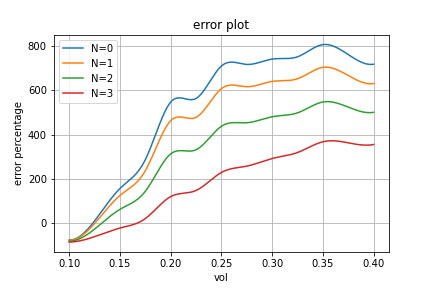
\includegraphics[width=0.5\textwidth]{./figures/T=0.5,K=0.15, kappa=6,m=0.06, sigma=1.4, gamma=1.2 error.png}\label{price diff9}}
  \caption{mean-reverting CEV model result 3}
  \small{Parameters are $K=0.15, \kappa=6, m=0.06, \sigma=1.4, \gamma=1.2$}
  \label{mrcev res3}
\end{figure}

\section{Volatility option prices under Heston puls CEV model}

For Heston plus CEV model,

$$
\begin{aligned}
  d V_t &=\kappa_1 \left(V^{\prime}_t - V_t\right) d t+\sigma_{1} \sqrt{V_t} d W_t \\
  d V^{\prime}_t &=\kappa_2\left(\theta -V^{\prime}_t\right) d t+\sigma_{2} V^{\prime \gamma}_t d W^{\prime}_t
\end{aligned}
$$

\noindent and our auxiliary model, square root mean-reverting model,

$$
d V_t=\kappa(m - V_t) d t+\sigma_0 \sqrt{V_t} d W_t
$$

\noindent our parameters are $r=0.05$, $K=0.15$, $\kappa_1=4$, $\kappa_2=2$, $\theta=0.2$, $\sigma_0=\sigma_1=0.3$, $\sigma_2=0.8$, $\gamma=1.6$, $\rho=0.5$ and different maturities $\tau=0.1$, $\tau=0.3, \tau=0.5$. We set the nuisance parameters $m= V^{\prime}(t)$, where $V^{\prime}(t)=0.2$ is the spot value for volatility of volatility at time $t$.

\begin{figure}[ht]
  \centering
  \subfloat[price comparison with $\tau=0.1$]{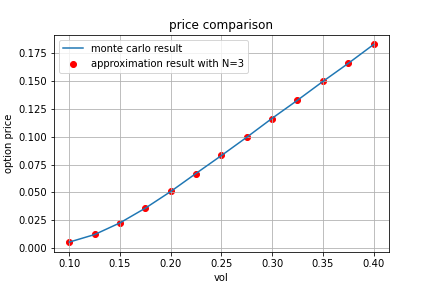
\includegraphics[width=0.5\textwidth]{./figures/heston cev rho=0.5,T=0.1,K=0.15, kappa=4,kappa2 =2,theta=0.2, sigma1=0.3,sigam2=0.8, gamma=1.6 price.png}\label{heston price comparison1}}
  \hfill
  \subfloat[relative error with $\tau=0.1$]{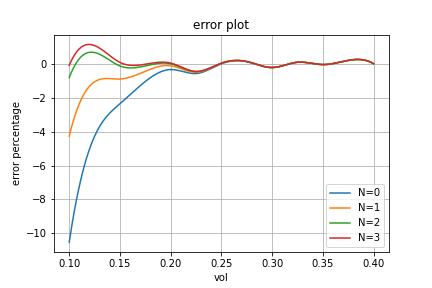
\includegraphics[width=0.5\textwidth]{./figures/heston cev rho=0.5,T=0.1,K=0.15, kappa=4,kappa2 =2,theta=0.2, sigma1=0.3,sigam2=0.8, gamma=1.6 error.png}\label{heston price diff1}} \\
  \subfloat[price comparison with $\tau=0.3$]{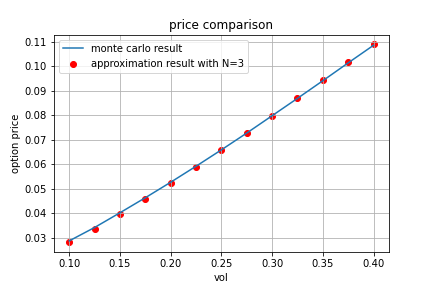
\includegraphics[width=0.5\textwidth]{./figures/heston cev rho=0.5,T=0.3,K=0.15, kappa=4,kappa2 =2,theta=0.2, sigma1=0.3,sigam2=0.8, gamma=1.6 price.png}\label{heston price comparison2}}
  \hfill
  \subfloat[relative error with $\tau=0.3$]{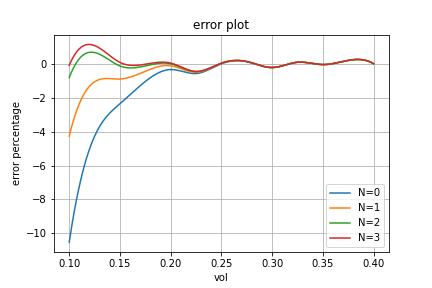
\includegraphics[width=0.5\textwidth]{./figures/heston cev rho=0.5,T=0.1,K=0.15, kappa=4,kappa2 =2,theta=0.2, sigma1=0.3,sigam2=0.8, gamma=1.6 error.png}\label{heston price diff2}} \\
  \subfloat[price comparison with $\tau=0.5$]{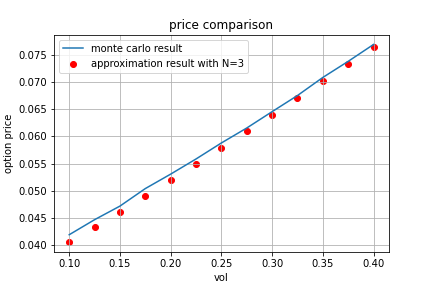
\includegraphics[width=0.5\textwidth]{./figures/heston cev rho=0.5,T=0.5,K=0.15, kappa=4,kappa2 =2,theta=0.2, sigma1=0.3,sigam2=0.8, gamma=1.6 price.png}\label{heston price comparison3}}
  \hfill
  \subfloat[relative error with $\tau=0.5$]{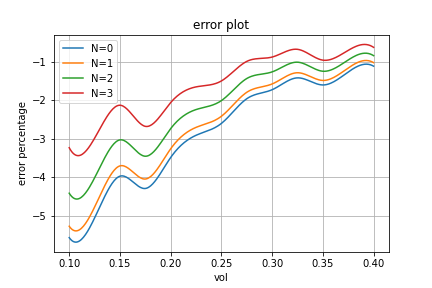
\includegraphics[width=0.5\textwidth]{./figures/heston cev rho=0.5,T=0.5,K=0.15, kappa=4,kappa2 =2,theta=0.2, sigma1=0.3,sigam2=0.8, gamma=1.6 error.png}\label{heston price diff3}}
  \caption{Heston plus CEV model result 1}
  \small{Parameters are $r=0.05$, $K=0.15$, $\kappa_1=4$, $\kappa_2=2$, $\theta=0.2$, $\sigma_0=\sigma_1=0.3$, $\sigma_2=0.8$, $\gamma=1.6$, $\rho=0.5$}
  \label{2d price comparison1}
\end{figure}

As is seen in figure \ref{2d price comparison1}, applying our method under 2-dimensional model can still create accurate results. Unlike mean-reverting CEV model, under Heston plus CEV model our relative differences are now converging to 0. This is because here the initial value of volatility doesn't enter mispricing function $\delta = \kappa_1(V_2-\theta_2) \Delta_{\bar{w}}$. We also test our method with $\rho=-0.5$, results are shown in figure \ref{2d price comparison2}.

\begin{figure}[ht]
  \centering
  \subfloat[price comparison with $\tau=0.1$]{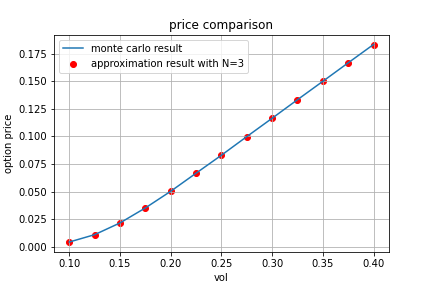
\includegraphics[width=0.5\textwidth]{./figures/heston cev rho=-0.5,T=0.1,K=0.15, kappa=4,kappa2 =2,theta=0.2, sigma1=0.3,sigam2=0.8, gamma=1.6 price.png}\label{heston price comparison4}}
  \hfill
  \subfloat[relative error with $\tau=0.1$]{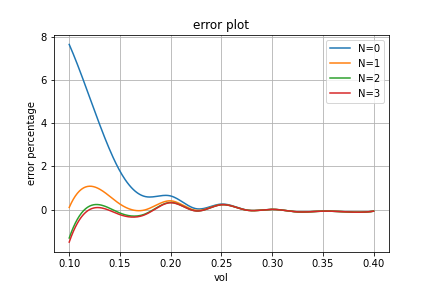
\includegraphics[width=0.5\textwidth]{./figures/heston cev rho=-0.5,T=0.1,K=0.15, kappa=4,kappa2 =2,theta=0.2, sigma1=0.3,sigam2=0.8, gamma=1.6 error.png}\label{heston price diff4}} \\
  \subfloat[price comparison with $\tau=0.3$]{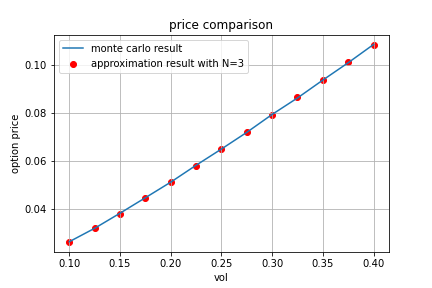
\includegraphics[width=0.5\textwidth]{./figures/heston cev rho=-0.5,T=0.3,K=0.15, kappa=4,kappa2 =2,theta=0.2, sigma1=0.3,sigam2=0.8, gamma=1.6 price.png}\label{heston price comparison5}}
  \hfill
  \subfloat[relative error with $\tau=0.3$]{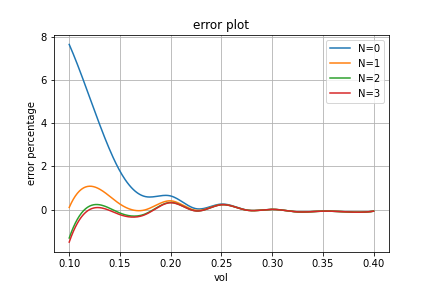
\includegraphics[width=0.5\textwidth]{./figures/heston cev rho=-0.5,T=0.1,K=0.15, kappa=4,kappa2 =2,theta=0.2, sigma1=0.3,sigam2=0.8, gamma=1.6 error.png}\label{heston price diff5}} \\
  \subfloat[price comparison with $\tau=0.5$]{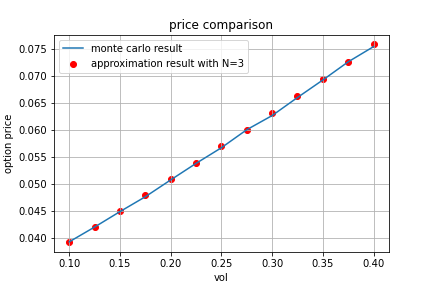
\includegraphics[width=0.5\textwidth]{./figures/heston cev rho=-0.5,T=0.5,K=0.15, kappa=4,kappa2 =2,theta=0.2, sigma1=0.3,sigam2=0.8, gamma=1.6 price.png}\label{heston price comparison6}}
  \hfill
  \subfloat[relative error with $\tau=0.5$]{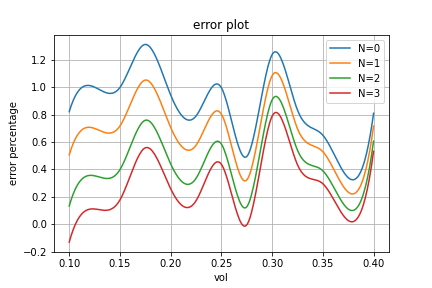
\includegraphics[width=0.5\textwidth]{./figures/heston cev rho=-0.5,T=0.5,K=0.15, kappa=4,kappa2 =2,theta=0.2, sigma1=0.3,sigam2=0.8, gamma=1.6 error.png}\label{heston price diff6}}
  \caption{Heston plus CEV model result 2}
  \small{Parameters are $r=0.05$, $K=0.15$, $\kappa_1=4$, $\kappa_2=2$, $\theta=0.2$, $\sigma_0=\sigma_1=0.3$, $\sigma_2=0.8$, $\gamma=1.6$, $\rho=-0.5$}
  \label{2d price comparison2}
\end{figure}

\chapter{Conclusion}\label{ch5}

In this thesis, we first review the approximation method proposed by \cite{heath_variance_2002} and \cite{kristensen_adding_2011}. Based on their work, we extend this method to price options under mean-reverting CEV model and the Heston plus CEV model. Selections of auxiliary models and corresponding mispricing functions are discussed. We also illustrate techniques to calculate partial derivatives of non-central chi-square distribution functions when using square root mean-reverting as the auxiliary model. Finally, we discuss our numerical results and explain the constraints of our method. In all, numerical results show that our method is efficient and accurate in most of the cases considered.